\begin{figure}[ht]
  \centering
  \begin{subfigure}{.49\textwidth}
    \centering
    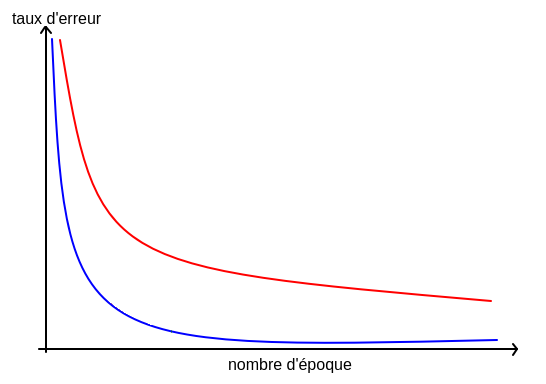
\includegraphics[width=.9\linewidth]{./Chapitre2/figures/surapprentissage2.png}
  \end{subfigure}
  \begin{subfigure}{.49\textwidth}
    \centering
    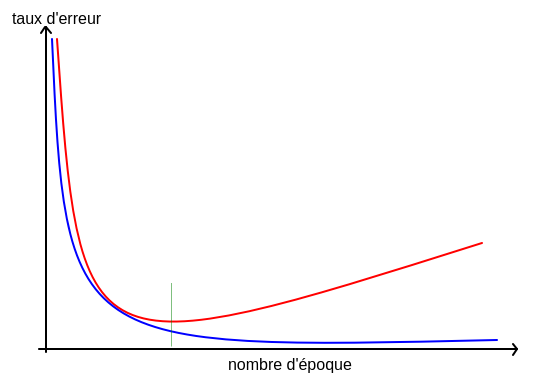
\includegraphics[width=.9\linewidth]{./Chapitre2/figures/surapprentissage1.png}
  \end{subfigure}
  \caption{Deux évolutions de scores sur les données d'entrainement en bleu et de développement en rouge. La figure de droite correspond à une situation de sur-apprentissage. Cette situation est observable à partir de l'époque correspondant à la ligne verte tracée.}
  \label{fig:surapprentissage}
\end{figure}
